%!TEX options = --shell-escape -8bit
\documentclass{article}
\usepackage{geometry}
\geometry{a4paper, scale=0.8}

\usepackage[utf8]{inputenc}
\usepackage{ctex}
\usepackage{assignpkg}
\usepackage{amsmath}
\usepackage{amssymb}
\usepackage{xcolor}
\usepackage[cache=false]{minted}
\studentIds{202XX80XXXXXXXX}{}
\studentNames{XXX}{}

\assignmentNumber{1}

\date{\today}

\begin{document}

% \makecover
\section*{课后作业} % (fold)
\label{sec:课后作业}
\subsection*{要求} % (fold)
\label{sub:要求}
	\begin{enumerate}
		\item 从两个高斯分布中采样。一组采样为正类,一组采样为负类。
		\item 编程实现\textcolor{blue}{线性回归,yi为-1或1。保存参数,画出回归投影面,同时可视化显示结果。}
		\item 编程实现\textcolor{blue}{线性判别分析,保留参数,对测试数据做出预测,同时可视化显示结果,画出分类面。}
		\item 实验1两个高斯分布具有一样的方差,实验2两个高斯分布具有不同的方差,观察实验结果的不同。
	\end{enumerate}
% subsection 要求 (end)
\subsection*{数据集生成代码} % (fold)
\label{sub:数据集生成代码}
\begin{minted}[
frame = single,
breaklines,tabsize=2,
baselinestretch=1,
linenos=false
]{python}
import numpy as np
import matplotlib.pyplot as plt


#生成训练数据集,每类100个数据
def get_train_data(data_size=100):
	data_label = np.zeros((2 * data_size, 1))# class 1
	x1 = np.reshape(np.random.normal(1, 0.6, data_size), (data_size, 1))
	y1 = np.reshape(np.random.normal(1, 0.8, data_size), (data_size, 1))
	data_train = np.concatenate((x1, y1), axis=1)
	data_label[0:data_size, :] = 0
	# class 2
	x2 = np.reshape(np.random.normal(-1, 0.3, data_size), (data_size, 1))
	y2 = np.reshape(np.random.normal(-1, 0.5, data_size), (data_size, 1))
	data_train = np.concatenate((data_train, np.concatenate((x2, y2), axis=1)), axis=0)
	data_label[data_size:2 * data_size, :] = 1
	
	return data_train, data_label


#生成测试数据集,每类10个
def get_test_data(data_size=10):
	testdata_label = np.zeros((2 * data_size, 1))
	# class 1
	x1 = np.reshape(np.random.normal(1, 0.6, data_size), (data_size, 1))
	y1 = np.reshape(np.random.normal(1, 0.8, data_size), (data_size, 1))
	data_test = np.concatenate((x1, y1), axis=1)
	testdata_label[0:data_size, :] = 0
	# class 2
	x2 = np.reshape(np.random.normal(-1, 0.3, data_size), (data_size, 1))
	y2 = np.reshape(np.random.normal(-1, 0.5, data_size), (data_size, 1))
	data_test = np.concatenate((data_test, np.concatenate((x2, y2), axis=1)), axis=0)
	testdata_label[data_size:2 * data_size, :] = 1
	
	return data_test, testdata_label
\end{minted}    
% subsection 数据集生成代码 (end)
\subsection*{训练集和测试集可视化结果} % (fold)
\label{sub:训练集和测试集可视化结果}
	\begin{figure}[H]
		\centering
		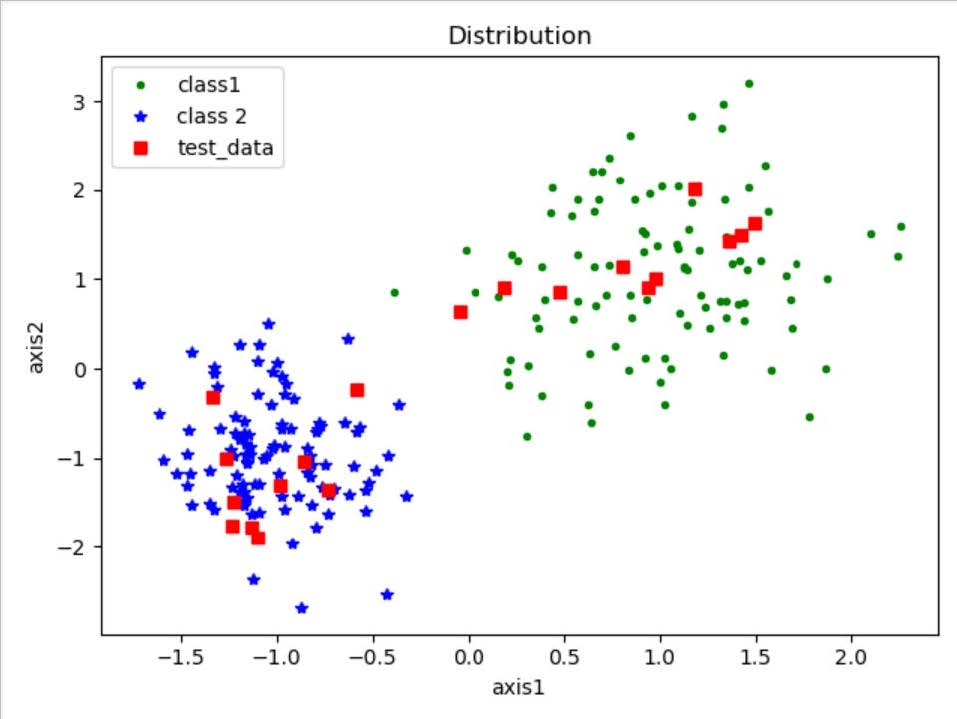
\includegraphics[width=0.8\textwidth]{Img/example.jpg}
	\end{figure}
% subsection 训练集和测试集可视化结果 (end)
% section 课后作业 (end)
\clearpage
\section*{解答} % (fold)
\label{sec:解答}
源代码见code/data.py
\subsection*{不同方差的两个高斯分布} % (fold)
\label{sub:不同方差的两个高斯分布}
	\begin{figure}[H]
		\centering
		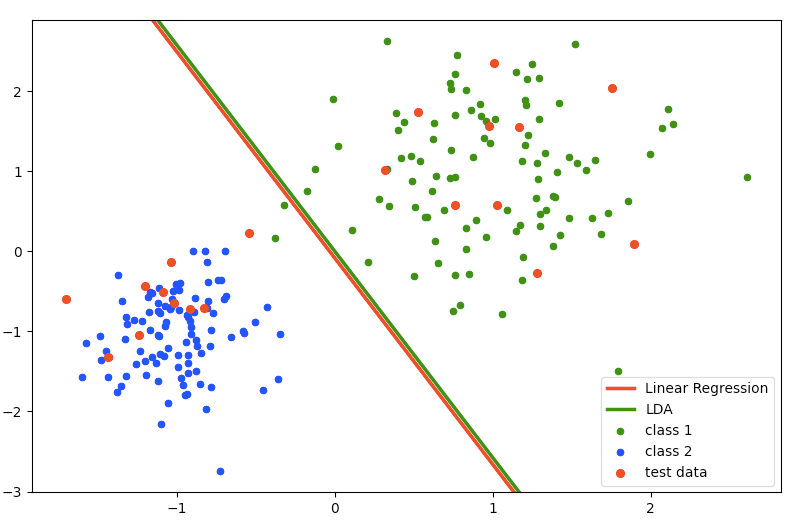
\includegraphics[width=0.7\textwidth]{Img/diff_train.png}
		\caption{训练}
	\end{figure}
	\begin{figure}[H]
		\centering
		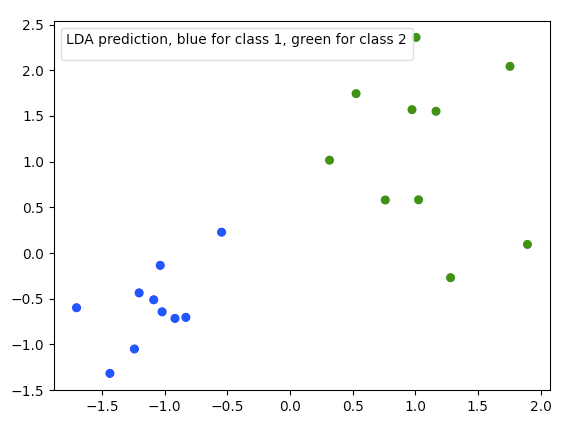
\includegraphics[width=0.8\textwidth]{Img/diff_predict.png}
		\caption{预测}
	\end{figure}

% subsection 不同方差的两个高斯分布 (end)
\subsection*{相同方差的两个高斯分布} % (fold)
\label{sub:相同方差的两个高斯分布}
	\begin{figure}[H]
		\centering
		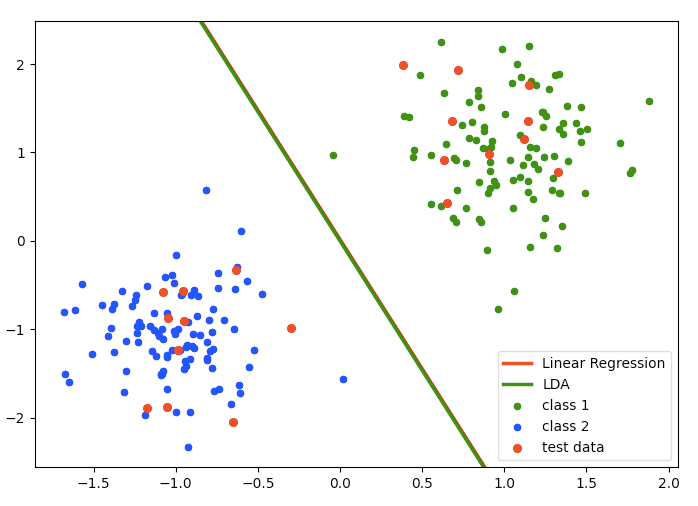
\includegraphics[width=0.8\textwidth]{Img/id_train.png}
		\caption{训练}
	\end{figure}
	\begin{figure}[H]
		\centering
		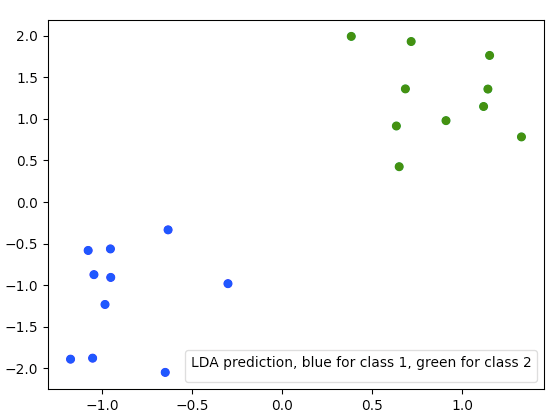
\includegraphics[width=0.8\textwidth]{Img/id_predict.png}
		\caption{预测}
	\end{figure}

% subsection 相同方差的两个高斯分布 (end)
% section 解答 (end)
\end{document}
